\chapter{综合监控总体设计}
\section{工程概况}
\subsection{线路背景}
\begin{figure}[h]
	\centering
	\includegraphics[width=0.4\textwidth]{地铁图标.png}
	\caption{地铁图标}
\end{figure}
天津轨道交通6号线(Tianjin Rail Transit Line 6)是中国天津市的第五条轨道交通线路。该线路于2016年8月6日首段工程(从长虹公园站至南翠屏站)开通运营,于2016年12月31日开通运营北段(从南孙庄站至长虹公园站),于2018年4月26日开通运营南段(从南翠屏站至梅林路站),并于2021年12月28日延伸至渌水道站。该线路的标志色为粉紫色。

天津轨道交通6号线呈半圆环形走向,东北起自东丽区的南孙庄站,途经河北区、红桥区、南开区、河西区、西青区,最终在津南区的渌水道站结束。它与天津轨道交通5号线形成了一个“O”型环线。

截至2022年1月,天津轨道交通6号线一期工程从南孙庄站至渌水道站的全长为43.43千米,其中地下线路为41.93千米,地上线路为1.5千米。该线路设有40座车站(其中北运河站尚未开通),其中包括1座高架站和39座地下站。此外,还设有大毕庄车辆段和尖山路地下停车线,列车采用6节编组B型列车。

在2016年8月6日,天津轨道交通6号线的客流量达到了1万人次。

需要特别说明的是,天津轨道交通8号线首通段(从渌水道站至咸水沽西站)目前以“天津轨道交通6号线二期工程”的名义运营,尽管实际上它包括了两条线路。"

\subsection{系统规模}

天津地铁6号线经估算全线接入的I/O总点数约为50万点。人机界面暂按1000张/站、5000张/中央级考虑,按照50个站点考虑系统容量,具体点数与人机界面在设计联络阶段最终确定。 

列表数据仅供参考,实际点表、数量在设计联络时确定。为了保证系统的性能和将来扩充,服务器、网络和软件平台的处理能力必须在上述基础上预留30\%以上的富裕量。 集成系统实时向综合监控系统传送数据,综合监控系统应支持查询和事件触发方式与集成系统交换数据。

\begin{table}[h]
	\centering
	\caption{典型车站(地下站)数据接入表}
	\label{tab:典型车站(地下站)数据接入表}
	
	\begin{tabular}{|c|c|c|}
		\hline
		序号 & 系统名称      & 单站接入点 \\ \hline
		1  & 电力监控系统    & 3000  \\ \hline
		2  & 环境与设备监控系统 & 4500  \\ \hline
		3  & 火灾自动报警系统  & 2000  \\ \hline
		4  & 屏蔽门系统     & 1000  \\ \hline
		5  & 其余系统(预留)  & 800   \\ \hline
		6  & 合计        & 11300 \\ \hline
	\end{tabular}%
\end{table}

\subsection{供电条件}
ISCS(智能监控与控制系统)是一级负荷供电系统,通过低压配电专业将两条独立的交流电源引入OCC(运营控制中心)、各车站和车辆段的综合监控设备室的交流配电柜,ISCS还负责实现这两路电源之间的自动切换。这两路电源采用三相五线制,电压为380/220V,波动范围在+10\%到-15\%之间,频率为50Hz $\pm$ 5Hz。

在OCC、各车站以及车辆段综合监控设备室,ISCS系统还设置了UPS电源设备,用来为ISCS、BAS(建策监控系统)、ACS(接入控制系统)、SPS(供电系统)以及车控室的各种专业设备提供不间断的220V交流电源。

此外,车站综合操作台的IBP(集成控制与电源系统)盘还需要配备开关电源转换模块,以实现从220V交流电源到DC24V电源的转换,以满足IBP盘本身和其他专业设备的电源需求。

在控制中心、各车站、车辆段和停车场,采用UPS方案,确保后备电源时间不少于1小时。此外,全线综合监控设备室的供电需要由动照专业提供两路市电交流电源(电压380V $\pm$ 15\%,频率50Hz)。动照专业负责在综合监控设备室内安装双电源引入箱,该引入箱采用壁挂方式安装于综合监控设备室内。小端的环控电控室的UPS电源则由动照专业提供。

\subsection{接地条件}
采用综合接地系统,确保接地电阻不超过1Ω。接地箱将由专业团队动照提供,并会放置在综合监控设备室和车站控制室内。投标人必须提供并安装ISCS系统至接地箱出线端子的接地线。
\subsection{环境条件}
根据天津地铁的环境特点和气候条件,充分考虑系统设备的抗电磁干扰、防尘、防潮、防霉、防震、防辐射等性能,确保系统运行安全、可靠。如\ref{tab:环境条件}所示。

% Please add the following required packages to your document preamble:
% \usepackage{multirow}
% \usepackage{graphicx}
\begin{table}[h]
	\centering
	\caption{环境条件}
	\label{tab:环境条件}
	
		\begin{tabular}{|cc|c|c|c|}
			\hline
			\multicolumn{2}{|c|}{项目}     & 控制中心      & 车站        & 轨旁及风道          \\ \hline
			\multicolumn{1}{|c|}{\multirow{3}{*}{\begin{tabular}[c]{@{}c@{}}温 度\end{tabular}}} & 工作 & 5℃〜+39℃ & 5℃$\sim$+39℃ & -31℃$\sim$+70℃ \\ \cline{2-5} 
			\multicolumn{1}{|c|}{} & 施工期 & 0℃〜+45℃   & 0℃〜+45℃   &                \\ \cline{2-5} 
			\multicolumn{1}{|c|}{} & 存储  & -25℃〜+50℃ & -25℃〜+50℃ & -25℃$\sim$+70℃ \\ \hline
			\multicolumn{1}{|c|}{\multirow{2}{*}{\begin{tabular}[c]{@{}c@{}}湿 度\end{tabular}}}       & 工作 & 5 〜90\% & 5 〜90\%      & 0 $\sim$100\%  \\ \cline{2-5} 
			\multicolumn{1}{|c|}{} & 存储  & 5 〜100\%  & 5 〜100\%  & 0 $\sim$100\%  \\ \hline
		\end{tabular}%
	
\end{table}

设计中的设备、元器件、材料必须满足以上的环境条件要求,具有高可靠的防潮、防腐、防锈、防尘等的性能,并在设备带电运行前,要有相应防护措施。

\section{系统集成和互联的对象}
综合监控系统采用以PSCADA、BAS、FAS为核心进行集成,兼顾部分与行车相关系统的集成和互联方案。

综合监控系统与SIG、AFC、ACS、UPS、PIS、CLK、PSD、ETC等系统进行互联,只接收相关信息,在必要的情况下,由HMI推出窗口显示,而不进行控制,相关设备工况显示及控制维护功能由其系统自行实现。综合监控系统预留与PA、CCTV互联条件。

\section{设计原则}

稳定性和安全性原则:系统的可靠性和安全性是远程监控系统成功实施的首要前提。设计方案应充分考虑业务需求对监控设备的不同使用要求。在设备选型方面,应优先选择经过验证的可靠、成熟的技术,以保障系统的稳定性、可靠性和安全性。我们的目标是构建一个稳定、可靠、安全的远程集中监控与管理系统。

合理性与易操作性原则:远程集中监控与管理系统的各子系统(如音视频监控录像系统、防盗报警系统、远程控制、远程语音对讲、远程网络传输系统)应具备相对独立运行的能力。接口应具有标准和通用特性,以确保各子系统能够完整集成和无缝连接,实现系统的有机合理、简洁维护以及相互联动。系统操作应采用中文界面,以保证易学易懂、简单操作。

先进性与实用性原则:设计方案应以实际需求为出发点,同时考虑满足现阶段的实时监控和录像记录需求,提供清晰准确的图像证据和实时远程图像传输等功能。还应考虑将来新技术的发展,以确保系统具备先进性和实用性。

完备性与扩展性原则:在设备选择上,应兼顾高清网络监控的实用性和可用性,同时考虑未来技术的发展、升级和扩容。系统应与现有系统融为一体,同时具备一定的前瞻性,以便将来融合新技术。随着IT技术的发展,系统应能够与未来的新技术相适应。

标准性与模块化原则:系统应采用模块化设计,以提供灵活性。当用户需求变化时,只需更换相应模块即可满足需求,实现方便的管理、使用和维护。

经济性与灵活性原则:在满足应用需求的前提下,应充分利用原有系统设备,降低成本。在系统布线方面,应满足各种应用需求,保持系统的灵活性。综合监控系统通过骨干网将综合监控系统中央监控网、车站级/定修段级监控网连接架构起整个网络系统。

\section{系统需求分析}
天津地铁6号线轨道交通1期工程综合监控系统包括控制中心ISCS系统、培训及仿真测试系统、网络管理系统(NMS),位于各车站、车辆段的车站级ISCS系统,位于车辆段的设备维修管理系统(DMS)等组成。重点是中心ISCS系统和各车站和车辆段的ISCS系统。

ISCS 系统为热备、全冗余、模块化、易扩展和高可靠性的系统。主、备机能实时地同时更新数据。当故障切换时,热备机能取代主机。这个原则适用于任何冗余设备,如服务器、FEP、网络设备、PLC、工作站等。系统能连续地自动检测系统的硬件和软件故障,故障时,切换自动进行。故障单元须被隔离,并且能建立一个新的有效的数据通道,使 ISCS 系统保持不间断工作。不间断工作的含义是,故障切换是无扰动的,切换过程中不能丧失系统监控功能,无误动作,数据记录不能中断和丢失。ISCS 系统的任何故障、电源故障或者故障切换不能引起被控系统设备的误动作或者切换。

ISCS系统由位于控制中心的中央级ISCS系统、培训管理系统(软件测试平台)、网络管理系统(NMS);各车站级、车辆段级、停车场级ISCS系统、车辆段的培训管理系统(培训系统)等组成。中央级、车站级ISCS系统采用主备、冗余、分层、分布式C/S结构,采用TCP/IP协议,并采用行之有效的故障隔离和抗干扰措施。现场级PLCS系统的PLC通过光纤自愈工业以太网环网或现场冗余双总线,将各类RI/O、具有智能通信口的现场设备和就地现场小型控制器等设备统一接入。

\subsection{控制中心}
中心ISCS是天津地铁10号线的综合监控系统之一,负责对车站、车辆段等地铁设备进行监控1。中心ISCS应实现综合监控系统集成和互联系统的中央功能,同时还应实现各系统间的中央联动功能。中心ISCS设计时需要预留与供电局地调、车载FAS、消防指挥中心、天津电梯安全运行处置中心、交通控制中心(TCC)等的接口,通过与通信上层网或直接接口,分别实现各接口功能。

由以太网交换机、服务器、FEP、工作站、打印机等部分组成。

\subsection{车辆段ISCS}
当中心ISCS或主干网出现问题时,车站ISCS要求不受影响,仍能工作。车站ISCS设计要求通过车站局域网络将现场级的信息汇集到车站级ISCS。干网和车站ISCS的连接需求为千兆网光口。

由以太网交换机、服务器、FEP、工作站、打印机等部分组成。

\subsection{车站ISCS}
当中心ISCS或主干网出现问题时,车辆段ISCS要求不受影响,仍能工作。车辆段ISCS设计要求通过车辆段局域网络将现场级的信息汇集到车站级ISCS,从而实现车辆段级的综合监控。车辆段ISCS与主干网之间也是需要通过冗余千兆光口进行连接。

综上所述,控制中心、车站和车辆段ISCS的需求分析各不相同,中心ISCS具有集成互联的中央、联动和接口功能需求。车站和车辆段ISCS具有汇集信息和干网连接的功能需求。

由以太网交换机、服务器、FEP、BPD盘、打印机等部分组成。关键设备选型如\ref{table:设备选型}所示:
\begin{table}[h]
	\centering
	\caption{天津地铁10号线轨道交通项目设备选型}
	\label{table:设备选型}
	\begin{tabular}{|l|l|l|}
		\hline
		\textbf{设备类型} & \textbf{型号} & \textbf{说明} \\ \hline
		以太网交换机 & Cisco Catalyst 9300 & 高性能企业级交换机 \\ \hline
		服务器 & Dell PowerEdge R740 & 适用于多功能环境的高性能服务器 \\ \hline
		前端处理器(FEP) & Advantech FEP-2150 & 工业级前端处理器,适用于复杂数据处理 \\ \hline
		BPD盘 & HPE StoreEasy 1660 & 高存储容量和备份功能的存储解决方案 \\ \hline
		打印机 & HP LaserJet Pro M404n & 高效率黑白激光打印机 \\ \hline
	\end{tabular}
\end{table}

\section{总体设计方案}
天津地铁6号线综合监控系统放弃了传统的集中式结构,创新地采用分层分布式、主备冗余结构,采用 TCP/IP 协议,具备有效的故障隔离和抗干扰措施。 

综合监控系统由安装在控制中心的中央级 ISCS,NMS,设置于车站、车辆段的 ISCS,设置于车辆段维修基地的设备维修管理系统,系统仿真测试平台等组成。

% TODO: \usepackage{graphicx} required
\begin{figure}[h]
	\centering
	\includegraphics[width=0.8\linewidth]{figures/ISCS系统构成图}
	\caption{ISCS系统构成图}
	\label{fig:ISCS系统构成图}
\end{figure}

\subsection{ISCS硬件构成}
第一层 - 中央级综合监控系统

包括冗余的实时服务器、冗余的历史服务器、外部磁盘阵列、磁带机、多种调度员工作站(如电调、环调、行调、维调和总调等)、NMS工作站、事件打印机、报表打印机、彩色图形打印机、带路由功能的冗余网络交换机、FEP、大屏幕系统(OPS)、UPS、WEB服务器、与更高一级指挥中心接口等。

第二层 - 车站级综合监控系统

第二层包括冗余的实时服务器、值班站长工作站、报表打印机、冗余的网络交换机、FEP、IBP和UPS等。车辆段综合监控系统(DISCS)与车站综合监控系统(SISCS)构成类似,但配置有所不同。FEP处理所有与被集成系统的接口,数据通过车站交换机传输至车站服务器。车站服务器、车站值班站长工作站和FEP等与网络交换机相连。

第三层 - 现场级 ISCS系统

即各子系统执行层面上的网络,包括PLCS、PSCADA、车站实时客流监测系统等分系统,采用工业控制以太网或现场总线。

\subsection{ISCS软件构成}
第一层 - 数据接口层

专门用于数据采集和协议转换,主要由综合监控系统前端处理器(FEP)构成,通过FEP的数据采集、协议转换、数据隔离等功能实现与相关系统的数据通信。

第二层 - 数据处理层

专门用于数据处理,主要由车站服务器和中央服务器构成,通过实时数据库和关系型数据库提供ISCS的应用功能。

第三层 - 人机接口层

专门用于处理人机接口,主要由操作员工作站构成,通过从车站和中央服务器获取数据,在工作站上显示人机界面。

控制中心系统和调度大厅系统设备组成如\ref{fig:控制中心机房系统设备组成图}和\ref{fig:调度大厅系统组成图}所示:

% TODO: \usepackage{graphicx} required
\begin{figure}[h]
	\centering
	\includegraphics[width=0.7\linewidth]{figures/控制中心机房系统设备组成图}
	\caption{控制中心机房系统设备组成图}
	\label{fig:控制中心机房系统设备组成图}
\end{figure}
% TODO: \usepackage{graphicx} required
\begin{figure}[ht]
	\centering
	\includegraphics[width=0.7\linewidth]{figures/调度大厅系统组成图}
	\caption{调度大厅系统组成图}
	\label{fig:调度大厅系统组成图}
\end{figure}



主要设备功能如下:

\begin{enumerate}
	\item 中央实时服务器:负责采集和处理实时数据,在OCC向各站点的集成系统发送控制命令,包括模式、程控和点控等。
	\item 中央历史服务器:用于存储、记录和管理历史数据。
	\item 磁盘阵列:作为数据存储设备,提高数据传输速率和安全性,并提供容错功能。
	\item 核心交换机:实现OCC内各网络资源的互连。需要根据ISCS和网络通信设备的要求,选择合适数量和带宽的交换机端口,直接与通信传输网络连接。
\end{enumerate}

\section{典型车站ISCS设计}

车站级综合监控系统(Station Integrated Supervisory Control System, SISCS)是一个高度先进的计算机系统,设计具备热备、冗余、开放、可靠和易扩展的特性。这个系统旨在连接特殊站点的车辆段综合监控系统(Depot Integrated Supervisory Control System, DISCS)和相邻车站的监控系统,并与主变电站相关的子系统集成。设备选型如\ref{典型车站ISCS设备选型}所示。
\begin{table}[h]
	\caption{典型车站ISCS设备选型}
	\label{典型车站ISCS设备选型}
	\centering
	\begin{tabular}{|l|l|c|}
		
		\hline
		\textbf{设备类型} & \textbf{设备选型} & \textbf{设备数目} \\
		\hline
		工业级以太网交换机 & Cisco Catalyst 9300 & 2 \\
		\hline
		实时服务器 & Dell PowerEdge R740 & 2 \\
		\hline
		前端处理器(FEP) & Siemens SIMATIC IPC & 2 \\
		\hline
		工作站 & HP Z4 G4 Workstation & 2 \\
		\hline
		报表打印机 & HP LaserJet Pro M404n & 1 \\
		\hline
		在线式后备电源(UPS) & APC Smart-UPS SRT & 1 \\
		\hline
		车站综合后备盘(IBP) & Custom Integrated Backup Panel & 1 \\
		\hline
	\end{tabular}
\end{table}



这些设备通过带路由功能的中央交换机接入全线骨干传输网。系统采用TCP/IP协议,符合IEEE802.3、IEEE802.3u及IEEE802.3ab/z标准。

在灾害或阻塞等特殊情况下,为确保中央级监控系统或车站级监控系统能持续运行,各车站控制室内配备了综合性的紧急后备盘(IBP)。IBP通过统一的远程I/O实现紧急情况下的后备控制功能,包括手动操作和显示,以确保安全。

紧急后备盘(IBP)的功能包括:

\begin{enumerate}
	\item 紧急停车、扣车和放行的SIG控制
	\item 环境控制通风排烟系统的紧急控制和消防联动
	\item PSD紧急开门控制
	\item AFC闸机释放控制
	\item 自动扶梯停止控制
	\item 门禁的门锁解锁
	\item 消防水泵启停等控制
\end{enumerate}

同时,IBP还提供时钟显示、重要系统的报警音响指示和指示灯测试等功能。车辆段综合监控系统不设置IBP,其后备手动操作与现实功能由FAS系统的联动控制盘完成。

车站的 ISCS 系统设备主要由两台站级服务器、两台交换机、KVM、两台站级工作站、UPS 等构成,站级设备自成一个小系统。当控制中心故障或与控制中心通信故障时,站级系统可以依靠自身完成对本车站内设备的监控功能,确保地铁安全运行。如\ref{fig:车站ISCS设备组成图}所示。

% TODO: \usepackage{graphicx} required
\begin{figure}[h]
	\centering
	\includegraphics[width=0.7\linewidth]{figures/车站ISCS设备组成图.pdf}
	\caption{车站ISCS设备组成图}
	\label{fig:车站ISCS设备组成图}
\end{figure}

\section{车辆段ISCS设计}
\textbf{1. 维护管理系统}

\begin{itemize}
	\item 维护管理系统分为两个部分,分别在车辆段维修中心和正线车站自动化工区实施。在车辆段维修中心,我们设置了一个维护管理系统(MMS),该系统用于采集、整合和处理综合监控系统所监控的主要设备的状态和故障信息。这些故障信息以单独设备故障报警的形式提供给车辆段维护管理人员,以协助他们进行日常设备维护工作。MMS系统通过交换机连接成局域网,然后通过网络端口接入综合监控系统的全线网络。在正线自动化工区,我们设置了车站工区维修系统,每个工区都可以收集本工区内各车站主要设备的状态和故障信息,以便正线工区维修人员进行指导和现场问题解决。
	
	\item 车辆段维护管理系统包括以下主要设备:
	\begin{itemize}
		\item 2 台以太网交换机(配置与站级以太网交换机相同)
		\item 2 套MMS服务器(配置与车站服务器类似)
		\item 1 套MMS外置磁盘阵列
		\item 2 台维修及复示工作站(PSCSDA、机电车间,配置与车站工作站类似)
		\item 3 台MMS工作站,配置与车站工作站相似,单屏显示(综合监控、BAS、PSCADA专业)
		\item 5 套维护管理便携式计算机
		\item 3 台MMS报表打印机(配置与车站报表打印机相似)
		\item 1 套UPS(配置与车站UPS相似)
	\end{itemize}
	
	\item 正线工区维修系统设在长陵站,维修工区包括以下主要设备:
	\begin{itemize}
		\item 1 套维修工作站(配置与车站工作站相似)
		\item 1 套维修便携式计算机
		\item 1 台维修报表打印机(配置与车站报表打印机相似)
	\end{itemize}
\end{itemize}

\textbf{2. 培训管理系统}

在车辆段的综合监控系统培训室内,我们设置了培训管理子系统(TMS),其目的是为学员提供一个模拟仿真的ISCS操作环境,以进行各种ISCS的培训操作,包括仿真单点设置、遥控、组控、模式控制等功能。TMS是一个独立的系统,配备了独立的培训系统软件,可以连接到综合监控系统网络,实现在线培训。

培训管理系统(TMS)包括以下主要设备:
\begin{itemize}
	\item 1 台培训系统以太网交换机(配置与站级以太网交换机相同)
	\item 1 台培训服务器(硬件配置与车站服务器类似,不考虑冗余)
	\item 4 台TMS工作站,其中包括 1 台培训教师工作站和 3 台学员工作站(配置与车站工作站相似)
	\item 1 套TMS专用的前端处理器(FEP)
	\item 1 台报表打印机(配置与车站事件打印机相似)
	\item 1 套相关系统的仿真模拟器
	\item 1 台投影仪
	\item 1 套专用培训管理软件
\end{itemize}

\textbf{3. 软件测试平台}

设置了一个软件测试平台(STP),它用于对相关系统的软件功能进行测试,以满足ISCS的软件安装测试和与各相关系统的接口测试要求。软件测试平台(STP)的硬件设备与培训管理系统的硬件基本相同,为了充分利用资源和节省投资,我们将软件测试平台与培训管理系统的硬件合并使用。它们分开配置,可以在不同的使用环境下安装不同的软件。同时,软件测试平台与综合监控系统监控网络相连接,以便于对全线综合监控系统的软件进行维护。

软件测试平台包括以下主要设备:
\begin{itemize}
	\item STP工作站(配置与车站工作站相同)
	\item 相关系统的仿真模拟器
\end{itemize}

车辆段的 ISCS 系统设备主要由车辆段综合监控、培训仿真和维修管理三个系统构成,完成对车辆段内所有设备的监视控制功能,如\ref{fig:车辆段ISCS设备组成图}所示:
% TODO: \usepackage{graphicx} required
\begin{figure}[h]
	\centering
	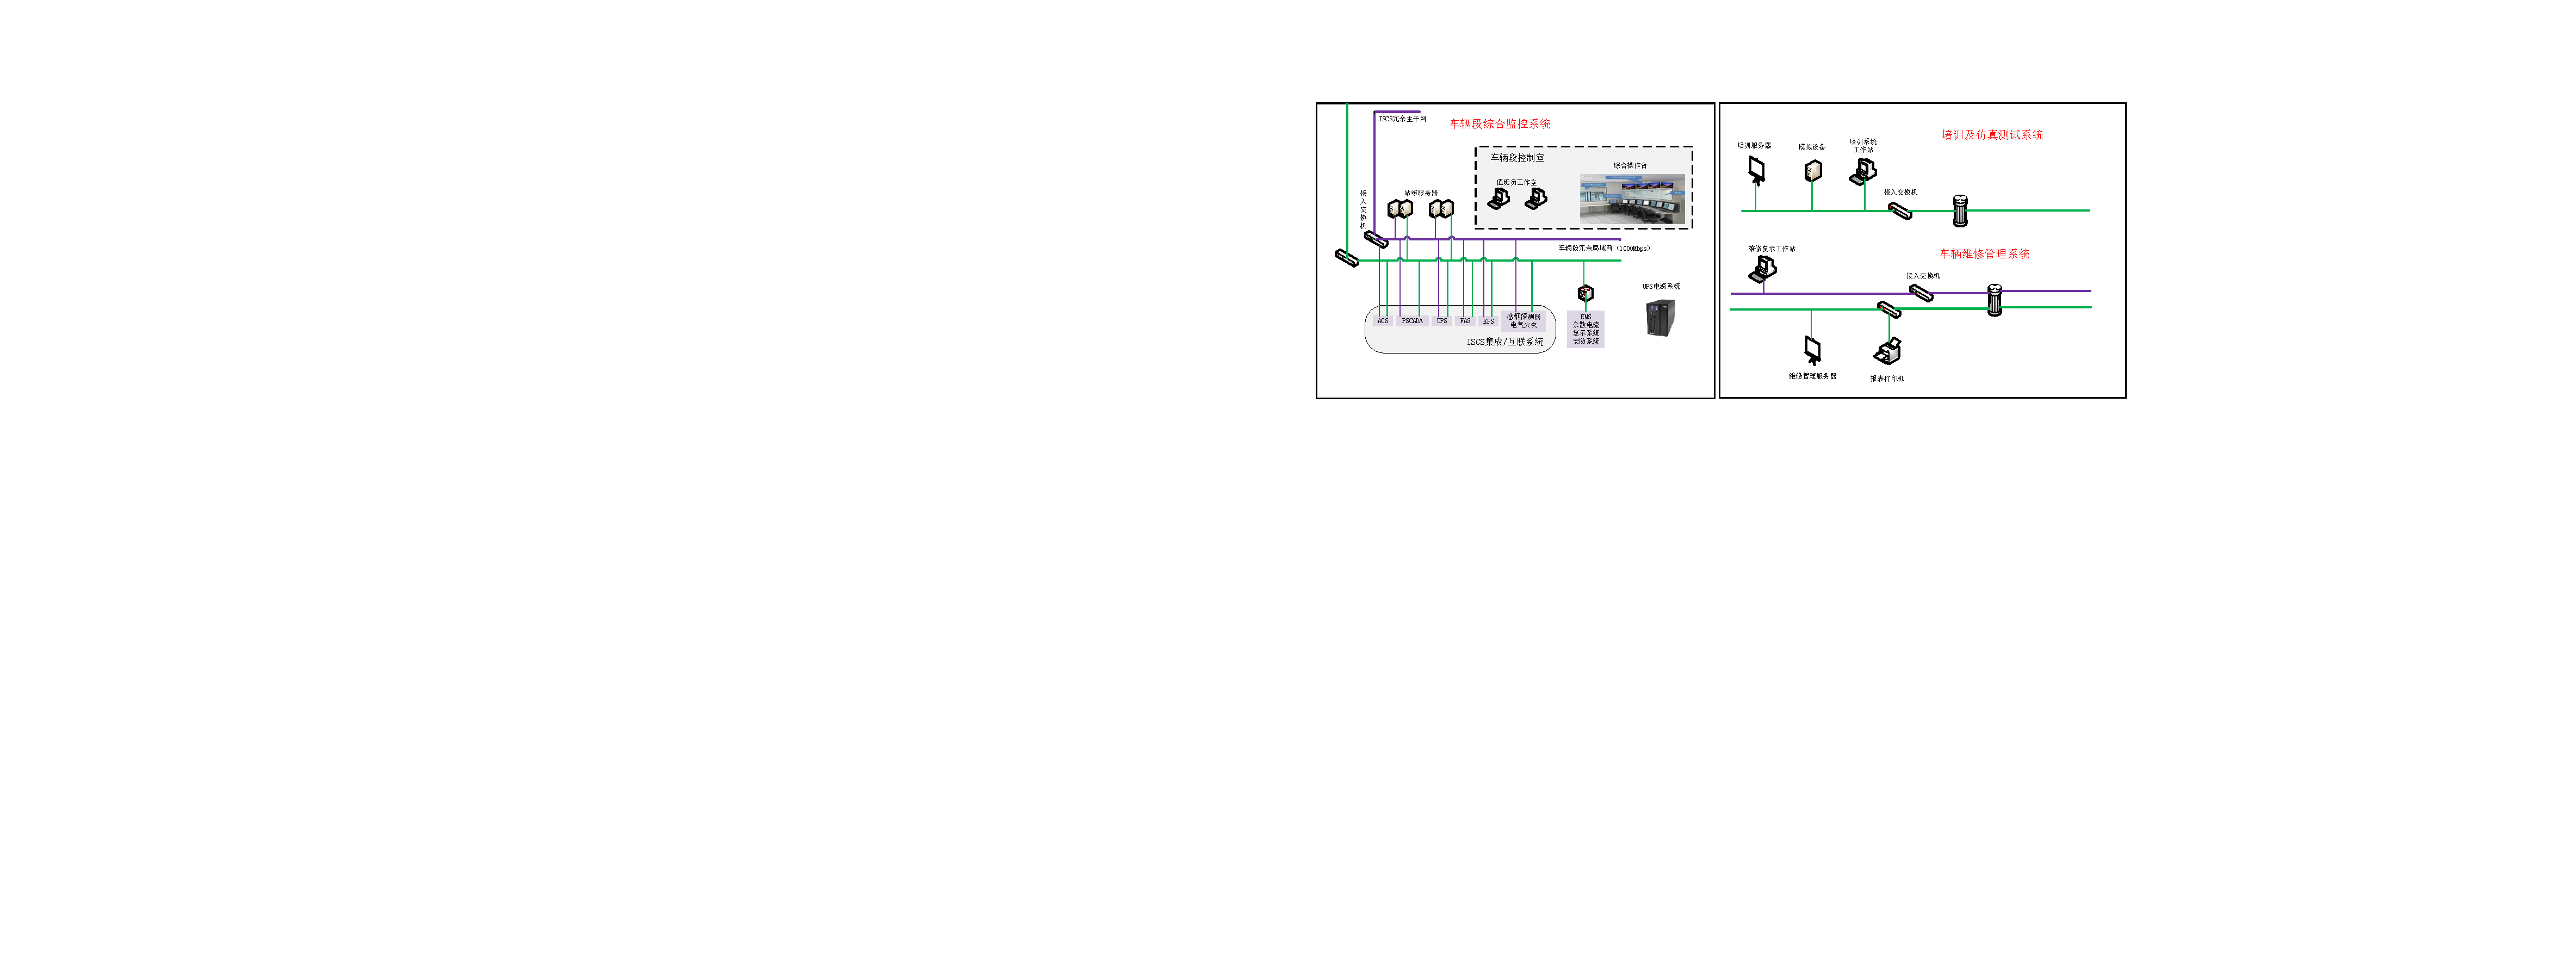
\includegraphics[width=0.8\linewidth]{figures/车辆段ISCS设备组成图}
	\caption{车辆段ISCS设备组成图}
	\label{fig:车辆段ISCS设备组成图}
\end{figure}


主要设备功能:

1. 培训仿真系统:系统提供以模拟相关系统规约到模拟现场环境的接口,教员在培训中能够修改仿真环境,并观察学员的响应,以在必要时提供建议。

2. 维修管理系统:实现对全线供电系统和机电设备系统复示和维修调度管理。

\section{系统网络设置}
天津地铁6号线线综合监控系统网络设计分为主干网络和站级网络两部分,主干网络实现中心、车站互联以及站内互联,站级网络实现 ISCS 与子系统的互联。
\subsection{骨干网组网方式}
骨干网网络拓扑结构设计为环型。骨干网网络由通信专业提供双环光纤资源,每个车站共八芯光纤到通信机房,接口为单模光纤,隔站跳接。



\subsection{主干网接入方式}
主干网络的拓扑结构采用分布式设计,其中逻辑结构是树型的,物理结构则呈星型。网络方案的设计如\ref{fig:主干网接入方式}所示。整个网络采用三层网络方案架构,每个车站都具有独立的AB双网,彼此之间完全隔离,互不干扰。此外,每个车站的网络通过三层路由协议划分为不同的网段,这种隔离设计能够确保一旦出现不可避免的故障,该故障只会影响到发生在该车站内的本系统,不会波及到其他部分网络。
% TODO: \usepackage{graphicx} required
\begin{figure}[h]
	\centering
	\includegraphics[width=0.5\linewidth]{figures/主干网接入方式}
	\caption{主干网接入方式}
	\label{fig:主干网接入方式}
\end{figure}

\subsection{站级网络结构}
站级网络实现综合监控系统与子系统的互联,其互联方式为交换机直连,如\ref{fig:站级网络结构}所示:
% TODO: \usepackage{graphicx} required
\begin{figure}[h]
	\centering
	\includegraphics[width=0.5\linewidth]{figures/站级网络结构}
	\caption{站级网络结构}
	\label{fig:站级网络结构}
\end{figure}

综合监控系统的详细设计涵盖了网络部分的规划。该系统依赖通信系统提供的通信通道来构建自己的通信骨干网络。在地铁的公共通信网络中,通信专业采用了MSTP网络,为综合监控系统提供了两条带宽为500M的通道。站级局域网由综合监控系统自身提供。考虑到综合监控系统需要实时监控各集成系统,并在突发事故时处理大量数据,网络的吞吐量必须足够大。为确保系统性能和未来扩展,服务器、网络和软件平台的处理能力都预留了50\%的冗余。此外,网络设备的处理能力和接口也考虑到了长期扩展的需求。

综合监控系统的主要功能是连接运营控制中心、车站和车辆段等局域网与OCC局域网之间的互联。每个车站、车辆段和运营控制中心都被视为网络节点,并使用主备冗余的千兆以太网三层交换机。所有车站、车辆段和运营控制中心的ISCS主要设备都连接到交换机上,以进行数据通信。通过通信传输通道,CISCS、SISCS和DISCS等集成子系统被连接成一个完整的监控系统。

综合监控系统的网络利用以太网交换机的虚拟局域网功能,将系统本身以及与其接口为以太网的相关接入系统划分为独立的虚拟子网。这种设计使得各集成子系统之间在逻辑上相对独立,并允许将各集成子系统划分为独立的虚拟维修子网,从而实现维修信息与监控信息的相对独立性。